\section{Traditional Distributed Computing Model}
\label{sec:traditional-distributed-computing}

Distributed computing systems are inherently distributed systems, which means
they share the fundamental characteristics and goals defined by
\citeauthor{tannenbaum2017} \cite{tannenbaum2017} as resource sharing,
transparent distribution, openness, and scalability. Distributed computing
facilitates distributed system principles in order to group a set of resources
(possibly at a geographical distance) and provide tenants with a single,
coherent view of these resources. In general, distributed computing systems
allow users to share, manage access to, and use compute, storage, and network
resources.

In the following two sections, we will look at two major distributed computing
concepts: Grid and Cloud computing.

\subsection{Grid Computing}

The Grid Computing model focuses on sharing widely distributed resources to
provide problem-solving environments and enable collaboration for a set of
individuals or institutions, so-called virtual organizations. It provides basic
mechanisms in the form of network protocols and interfaces that offer means of
discovering, managing access to, and using remote resources. Because those
resources are not subject to centralized control, these protocols and interfaces
must be standardized and open to enable interoperability \cite{foster2001grid}.

The hourglass model facilitated by the internet protocol stack can also be found
in the Grid computing architecture. While the base of the hourglass provides
various fundamental behaviors, the neck defines a small set of abstractions,
allowing a diverse set of high-level behaviors to be built on top. The five
layers of the Grid computing model defined by \citeauthor{foster2001grid}
\cite{foster2001grid} are as follows:

\begin{figure}[H]
  \centering
  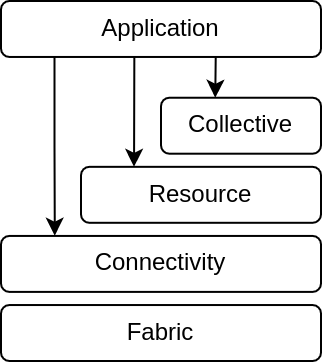
\includegraphics[width=0.25\linewidth]{resources/grid-architecture.drawio.png}
  \caption{The layered Grid architecture.}
  \label{fig:grid-architecture}
\end{figure}

\begin{description}
  \item[Fabric Layer]
    The fabric layer provides the resources which are shared by the Grid system.
    It offers local, resource-specific operations called by sharing processes at
    higher layers. These operations provide resource inquiry and management
    capabilities.

  \item[Connectivity]
    This layer specifies core communication protocols, enabling the exchange of
    data between fabric layer resources. Commonly includes transport, routing,
    naming, authentication, and authorization protocols.

  \item[Resource]
    On top of the connectivity layer, the resource layer defines protocols
    providing secure negotiation, initiation, monitoring, control, accounting,
    and payment mechanisms for individual resources. It facilitates fabric layer
    functions to access and control resources. These protocols are focused on
    single resources, meaning they are not concerned with coordinating multiple
    resources.

  \item[Collective]
    While the resource layer provides interactions with a single resource, the
    collective layer focuses on interactions with a collection of resources.
    Being the top of the hourglass allows this layer to provide a wide variety
    of behaviors, such as discovering, co-allocating, scheduling, brokering,
    monitoring, and replicating resources.

  \item[Applications]
    The final layer of the Grid architecture is the collection of user
    applications. These applications implement specific business logic by
    utilizing resources and services of the previous layers.
\end{description}

\subsection{Cloud Computing}

Cloud Computing systems typically have centralized control and facilitate open
and proprietary protocols and interfaces to provide on-demand self-service,
broad network access, resource pooling, rapid elasticity, and measured services.
\citetitle{mell2011} \cite{mell2011} defines three distinct service models of
Cloud computing:

\begin{description}
  \item[Infrastructure as a Service (IaaS)]
    In an IaaS service model, the managed resources are fundamental computing
    resources. This includes physical or virtual machines, storage, and
    networks. The consumer neither manages nor controls the underlying
    infrastructure but can deploy and run arbitrary software on the provided
    infrastructure, including system software such as operating systems.

  \item[Platform as a Service (PaaS)]
    The PaaS service model adds another layer of abstraction on top of the IaaS
    service model. Consumers can deploy and run applications on a provided
    platform that supports a set of programming languages, libraries, services,
    and tools. The consumer can run arbitrary applications supported by the
    platform but neither manages nor controls the provided platform services.

  \item[Software as a Service (SaaS)]
    The SaaS service model again adds another layer of abstraction. Compared to
    the PaaS model, the consumer can not run arbitrary applications but only a
    provider-specific selection of applications. Furthermore, the Cloud provider
    controls and manages the applications, only allowing customers to customize
    a limited set of user-specific configurations.
\end{description}

These service models can be seen as hierarchical layers providing various
resources and service, which customers can utilize to develop and deploy
applications.

\subsection{Trust Model}

There are three roles that are present in the traditional distributed computing
model.

\begin{description}
  \item[Service Provider]
    Generally, a service provider is an entity or organizational unit that
    provides services to other entities or organizational units. In the
    distributed computing context, service providers provide application and
    data owners with infrastructure resources and/or platform services.

  \item[Application Owner]
    Application owners manage applications that operate on data owned by the
    data owner. This does not imply that the application owner develops
    applications. Applications can be developed and provided by separate
    entities.

  \item[Data Owner]
    Data owners are in the possession of data that is being used or manipulated
    by an application. They are concerned about the confidentiality of their
    data. There may be mutual distrust between data owners if there are multiple
    data owners.
\end{description}

This trust model needs to be applied from the perspective of the data owners and
is tied to a set of data. For example, in a Grid environment, three virtual
organizations $A$, $B$, and $C$, share resources and services. Assuming that
virtual organization $A$ owns dataset $D$ but all of $A$'s resources are
currently occupied. Therefore, $A$ wants to use resources from virtual
organization $B$ to run an application on dataset $D$. In this context, while
all virtual organizations share resources, only $B$ takes on the role of a
service provider because $A$ does not share resources used for this specific
context and $C$ is not involved at all. Because $A$ manages the application and
owns the dataset $D$, $A$ takes on the role of application owner and data owner
in this example.

Traditionally, the data owner trusts the application owner and service
providers. Therefore, both roles can be taken on by the same party.

\subsection{Architectural Overview}
\label{sec:traditional-architecture-overview}

\begin{figure}[H]
  \centering
  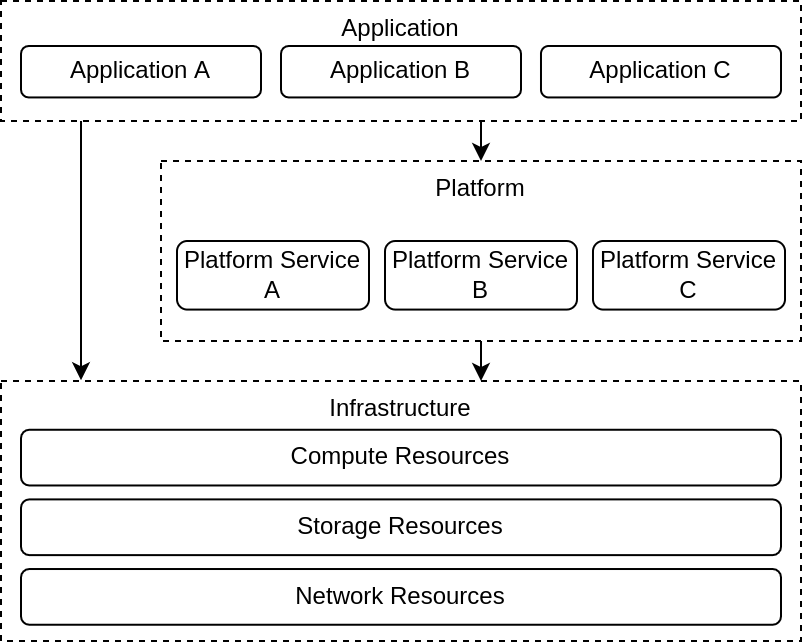
\includegraphics[width=0.7\linewidth]{resources/distributed-computing-overview.drawio.png}
  \caption{Layered model of a distributed computing system.}
\end{figure}

This section defines a generalized distributed computing model architecture,
consisting of three layers:

\begin{description}
  \item[Infrastructure]
    This layer provides fundamental resources, such as compute, network, and
    storage resources. This commonly includes physical or virtual machines
    (compute resource), layer two or three networks connecting machines (network
    resource), and network attached storage (storage resource).

    In the Cloud model, this layer corresponds to the IaaS service model and in
    the Grid architecture it is represented by the fabric layer.
  \item[Platform]
    The platform layer sits between the infrastructure and application layer. It
    provides a set of services and tools that support application owners to run
    applications in a distributed computing environment and manage the
    underlying infrastructure resources required for the application to run. The
    platform layer abstracts the complexity of the underlying infrastructure by
    providing services to manage, access, and utilize needed resources. These
    services are all operated and provided by the service provider.

    This layer matches the Cloud's PaaS and SaaS service model and is
    represented by the collection of the resource, connection, and collective
    layer in the Grid architecture.
  \item[Application]
    The final layer is the collection of applications and services managed by
    application owners.
\end{description}

In the following figures, components of the infrastructure layer are marked in
blue, the platform layer in red, and the application layer in green.

\subsubsection{Infrastructure Layer}

\begin{figure}[H]
  \centering
  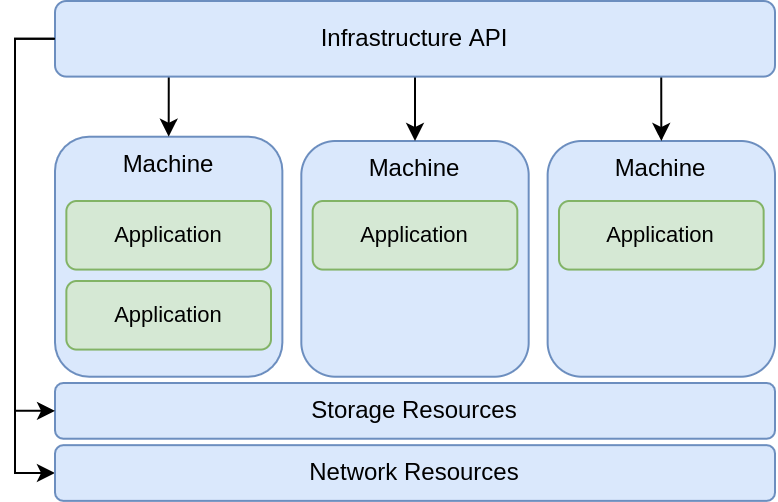
\includegraphics[width=0.6\linewidth]{resources/distributed-computing-infrastructure-example.drawio.png}
  \caption{Overview of the infrastructure layer in the traditional distributed computing model.}
  \label{fig:traditional-infrastructure-overview}
\end{figure}

While various kinds of user interfaces can be provided to tenants, such as
websites, web portals, terminal user interfaces, graphical user interfaces,
software development kits, and libraries, these user interfaces generally
facilitate an application programming interface (API) that exposes resource
management actions. To keep this model general, this model assumes the presence
of an API.

Typically, computing resources provided by the infrastructure layer are in the
form of machines, which combine CPUs, memory, peripheral devices, and ephemeral
(machine-local) storage. Storage and network resources can be provided in
various forms, such as block-level, file-level, and object-level storage, and
layer two and three networks. While compute resources provide execution
environments for applications, storage resources allow storing data independent
of a machine's lifecycle, and network resources enable connectivity between
infrastructure resources. To keep this model abstract, we will not make any
assumptions about the specifics of storage and network resources.

However, infrastructure resources can be provided in two forms: physical or
virtual. Protection of data in physical infrastructure resources can be
implemented for example by securing the physical location of the hardware, and
facilitating application transparent encryption. Virtual infrastructure is
protected by the isolation that virtualization systems, such as hypervisors,
provide. This requires a correctly configured and actively patched
virtualization system, as misconfiguration can lead to breaking the isolation
guarantees, and not patching virtualization systems allows attackers to exploit
vulnerabilities. For example, hypervisors are large pieces of software that
require complex configuration, and over the years, numerous vulnerabilities have
been found in commonly used hypervisors
\cite{perezbotero2013hypervisorvulnerabilities,
reuben2007surveyvirtualmachinesecurity}.

Because the service provider manages the physical hardware and virtualization
systems, the protection of infrastructure layer resources is entrusted to the
service provider.

\subsubsection{Platform Layer}

The platform layer offers various kinds of services. Commonly found services
are:

\begin{description}
  \item[Resource management]
    Management of compute and storage resources. This could include the ability
    to monitor, allocate, and release resources to scale dynamically depending
    on the current needs.
  \item[Authentication and authorization]
    Provide ways to verify the identity of a user or process and define and
    enforce policies governing the access to infrastructure resources and
    applications.
  \item[Messaging and communication]
    While the infrastructure provides basic infrastructure for communication by
    providing network resources, the platform layer often provides higher level
    communication such as inter-process communication, message passing, and
    event notifications.
  \item[Data management]
    Provide means for storing and accessing data by managing storage resources
    of the infrastructure layer. Often includes caching, replication, and
    synchronization services to maximize availability, integrity, and
    performance.
  \item[Service discovery and load balancing]
    Expose applications as network services to other applications and
    distributing traffic to multiple instances of an application.
  \item[Monitoring and logging]
    Support the monitoring of applications for failures and performance issues
    and aggregate logs of applications for debugging and auditing purposes.
  \item[Collaboration frameworks]
    Provide problem-solving environments that manage multistep, asynchronous,
    multi-component workflows.
  \item[Application deployment]
    Decrease the burden of deploying applications, providing mechanisms to
    deploy and configure applications in execution environments.
  \item[Key Management]
    A Key Management Service (KMS) manages cryptographic keys used to encrypt
    and decrypt confidential data. These services typically provide mechanisms
    for generating, storing, and providing keys to other applications and
    services.
\end{description}

While these services implement various types of behaviors, they can be grouped
into five non-mutually exclusive categories:

\begin{description}
  \item[Infrastructure management]
    Services that manage infrastructure layer resources to automate the
    management and simplify access to those resources. They often also provide
    more complex behaviors like data management, application-level
    communication, service discovery, and load balancing. These services need
    the privilege to allocate, release, and monitor infrastructure resources.

  \item[Security]
    Services that offer application-level authentication, authorization, and
    encryption to ease the process of implementing security into an application.
    These services manage the identities of applications and users, control
    access to resources and services, and generate and manage cryptographic
    keys.

  \item[Monitoring and Logging]
    Monitoring and logging services collect monitoring metrics and logs from
    applications.

  \item[Application orchestration]
    Application orchestration refers to the automated management of
    applications. This involves the preparation of target execution environments
    and installing, configuring, and executing applications inside the target
    environments.
\end{description}

The usage of platform layer services provided by a service provider is optional.
Application owners can manually manage infrastructure layer resources, collect
logs and metrics, and orchestrate applications or implement those services in
the application layer. But because the service provider is assumed to be
trusted, it is often in the interest of the data and application owner to
facilitate services provided by the service provider to automate specific
processes, be more cost-efficient, and reduce the complexity of the application
layer.

\subsubsection{Application Layer}

The final layer is the application layer, consisting of the application owners'
applications. These applications can also be in the form of services typically
located in the platform layer and managed by the service provider. For example
the application owner can choose to manage its own security service that
provides authentication, authorization, and encryption to other applications.

The main distinction between the application layer and the platform layer is
that the application owner manages the applications of the application layer,
while the service provider operates the platform layer services.

\subsection{Example: Kubernetes in a Cloud Environment}
\label{sec:example-kubernetes}

Kubernetes is an extensible, open-source platform for managing containerized
applications. Due to its open-source nature and popularity, the ecosystem
surrounding Kubernetes has been rapidly growing. It provides general platform
services that fall in the infrastructure management and application
orchestration categories, with the ability to integrate with monitoring and
logging solutions. While Kubernetes provides the services of the platform layer,
it manages applications on top of a separate infrastructure layer, such as a
Cloud IaaS offering.

Commonly used Cloud providers such as Amazon Web Services (AWS), Microsoft
Azure, and Google Cloud Platform (GCP) offer a managed Kubernetes service (AWS
Elastic Kubernetes
Service\footnote{\url{https://docs.aws.amazon.com/eks/index.html}}, Azure
Managed Kubernetes
Service\footnote{\url{https://learn.microsoft.com/en-us/azure/aks/}}, Google
Kubernetes
Engine\footnote{\url{https://cloud.google.com/kubernetes-engine/docs}}),
providing both infrastructure resources and platform services.

In this example, the Cloud provider takes on the service provider role.

\begin{figure}[H]
  \centering
  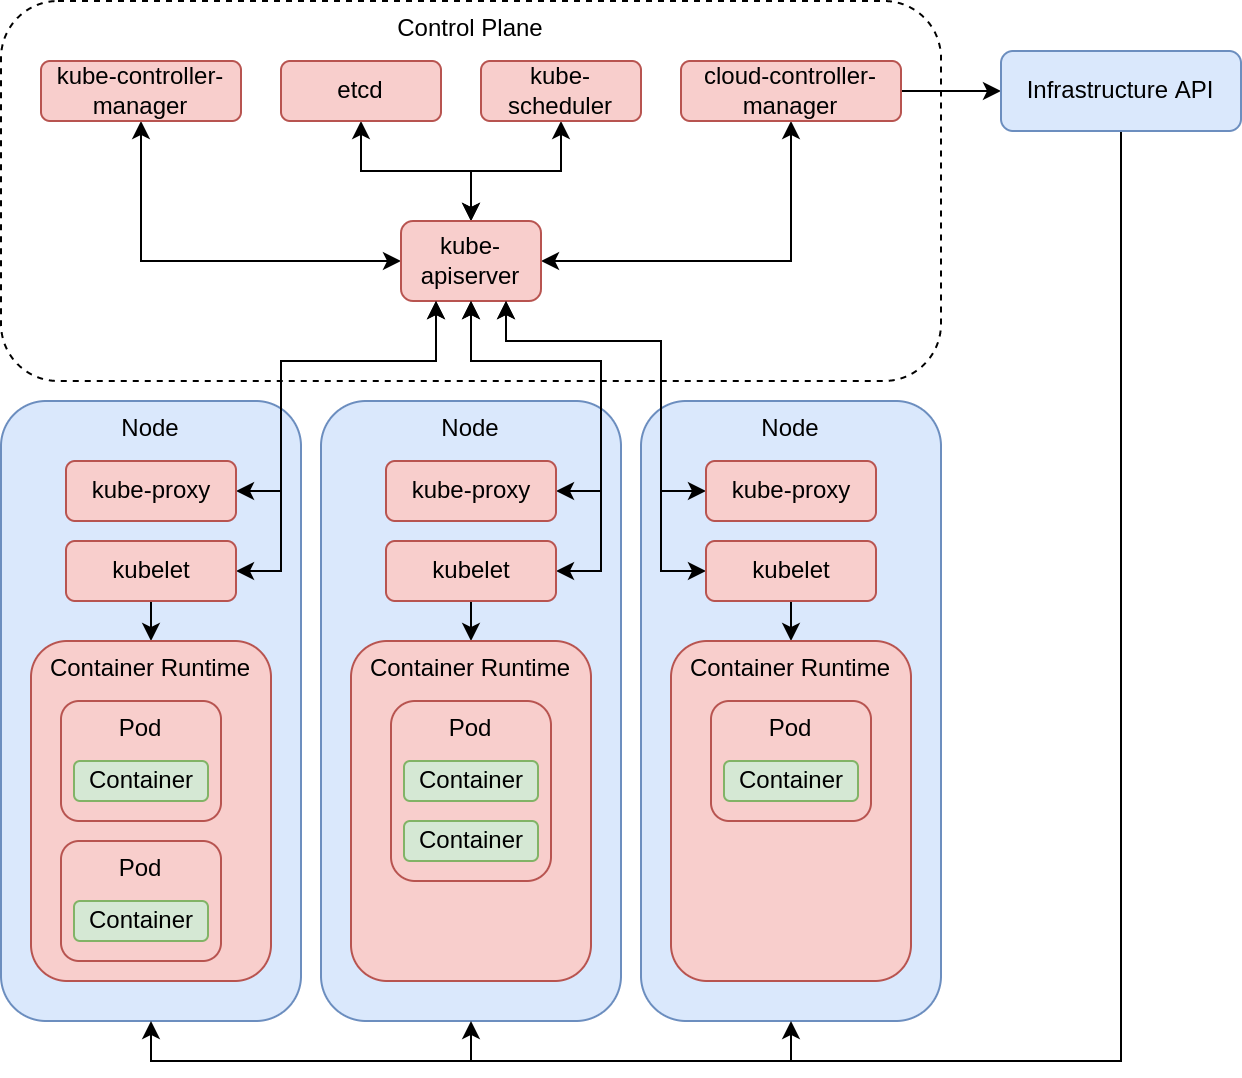
\includegraphics[width=0.8\linewidth]{resources/kubernetes-overview.drawio.png}
  \caption{Overview of core Kubernetes components.}
  \label{fig:kubernetes-overview}
\end{figure}

We will first look at an overview of the components of a Kubernetes cluster.
Figure \ref{fig:kubernetes-overview} can assist the reader in understanding the
relations between those components.

\begin{description}
  \item[Pods]
    A group of containers that share storage and network resources that models
    an application-specific logical host. The containers that make up a pod are
    always located on the same node and are scheduled in unison.

    In a broader sense, pods are logical execution environments in which
    applications, in the form of containers, can be deployed and executed. As
    such, pods are managed execution environments of the platform layer that
    contain application containers of the application layer.

  \item[Nodes]
    Nodes are machines running containerized applications. The following
    components are present on each node: kubelet, container runtime, and
    kube-proxy. The kubelet is an agent that is responsible for making sure that
    all containers of a pod are running, while the container runtime is the
    software that is responsible for running containers. Kube-proxy is a network
    proxy that implements the discovery of applications inside the cluster and
    the exposure of those applications as network services.

    Nodes correspond to compute resources of the infrastructure layer. However,
    the components on those nods implement application orchestration and
    infrastructure management capabilities and are part of the platform layer.

  \item[Control Plane]
    A collection of components that manage nodes and pods inside the cluster,
    making global decisions about the cluster. This includes an API
    (kube-apiserver), a backing store for all cluster data (etcd), and a
    scheduler (kube-scheduler) that assigns pods to nodes. Kubernetes adopts the
    concept of control loops, enabling the use of so-called controllers, which
    are non-terminating loops that watch the state of the cluster and make
    requests for changes when needed. While each controller is a logically
    separate process, they are compiled into a single kube-controller-manager
    component.
    
    The management of infrastructure layer resources is abstracted by the
    cloud-controller-manager, which implements Cloud specific resource
    management. All control plane components are also deployed in the Kubernetes
    cluster using pods.
    
    The control plane stores the desired global state of the cluster and
    requests modifications of the cluster to reach the desired state upon
    request of a tenant or change of the actual cluster state. These
    modification requests are either processed by another control plane
    component, such as the cloud-controller-manager allocating a new node by
    calling the infrastructure layer API, or components on existing nodes, such
    as the kubelet creating a new pod.
\end{description}

\subsubsection{Infrastructure Management}

Kubernetes enables Cloud providers to implement Cloud specific infrastructure
management services by developing a cloud-controller-manager, Container Storage
Interface (CSI) plugins, and Container Network Interface (CNI) plugins, allowing
tenants to automatically scale their Kubernetes cluster depending on the current
need.

The cloud-controller-manager typically consists of multiple components that
manage the lifecycle of nodes and load balancers.

CSI plugins are responsible for creating, updating, and destroying storage
resources in order to provide pods with persistent storage, referred to as
persistent volumes. Cloud providers often also provide storage encryption in
conjunction with their storage resources. These encryption services use keys
provided by a KMS. While some Cloud providers allow tenants to utilize their
self-managed KMS, the encryption service still needs plain text access to keys
to encrypt and decrypt data.

CNI plugins create, update, and destroy the underlying network resources of the
Kubernetes cluster and provide node-level, and pod-level communication. Some CNI
plugins also allow tenants to enforce network policies in the cluster, and
transparently encrypt data traversing the network resources in order to protect
confidential data.

\subsubsection{Application Orchestration}

The basic workflow of how Kubernetes orchestrates application containers on
nodes is as follows. Note that this description of the workflow is greatly
simplified.

\begin{figure}[H]
  \centering
  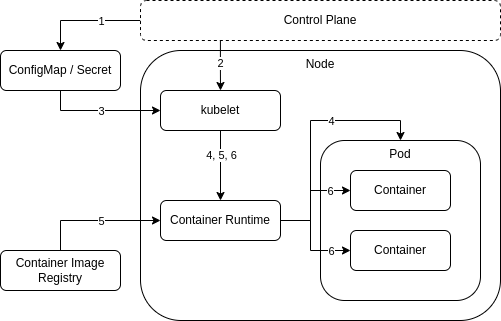
\includegraphics[width=0.7\linewidth]{resources/kubernetes-application-orchestration.drawio.png}
  \caption{Kubernetes' application deployment, configuration, and execution workflow.}
  \label{fig:kubernetes-application-orchestration}
\end{figure}

\begin{enumerate}
  \item Upon request of a tenant, the control plane creates ConfigMaps/Sects,
        which contain non-confidential/confidential configurations of an
        application.
  \item Upon request of a tenant, the control plane requests the kubelet of a
        node to create a pod and provides the kubelet with the specification of
        the pod. This specification includes container images,
        ConfigMaps/Secrets, storage configuration, and network configuration.
  \item Kubelet pulls specified ConfigMaps/Secrets onto the node.
  \item Kubelet calls the container runtime to create the pod, configure its
        storage and network, and provide the pod with the configurations of the
        ConfigMaps/Secrets.
  \item Kubelet calls the container runtime to pull the specified container
        images.
  \item Kubelet calls the container runtime to create and start the application
        containers inside the pod using the pulled container images.
\end{enumerate}
